%Conclusion body
%Created MB 04-12

\section{Analysis}\label{analysis}
\subsection{Second Sound Analysis}\label{analysis}

By analyzing the second sound data shown in Figure \ref{fig:secondsoundraw}, we can determine the relationship between the temperature of He II and the propagation speed of second sound.  By using linear regression analysis, we can determine the slope of each data set corresponding to a certain He II temperature.  For each of the fifteen data sets, the coefficient of determination, $r^{2}$ is greater than $0.99$.  The values for the slope of these fits, in m/s, correspond to the propagation speed of second sound in the respective temperature.  These speeds can then be plotted against temperature in order to show the relationship between the two in He II.  Due to the goodness of each fit, the statistical error in the data is smaller than each speed's level of precision. Figure \ref{fig:secondsound} shows the relationship between second sound speed and temperature in He II.  This data is compared to results made by Peshkov.\cite{peshkov}

In order to eliminate systematic error in second sound calculations, we chose not to calculate velocity by simply dividing a measured displacement between the balometer from the heater by an observed time delay between the pulse trigger and signature recorded by the balometer. This method would insert systematic offsets to either the time delay or the displacement which would then affect the overall accuracy of second sound speeds.  By calculating the slope of several of these measurements we remove the effect of these offsets and instead emphasize the relative differences between data points.  As a result, the error in second sound speed is purely statistical given by the linear regression analysis.  


\begin{figure}[htbp]
\begin{center}
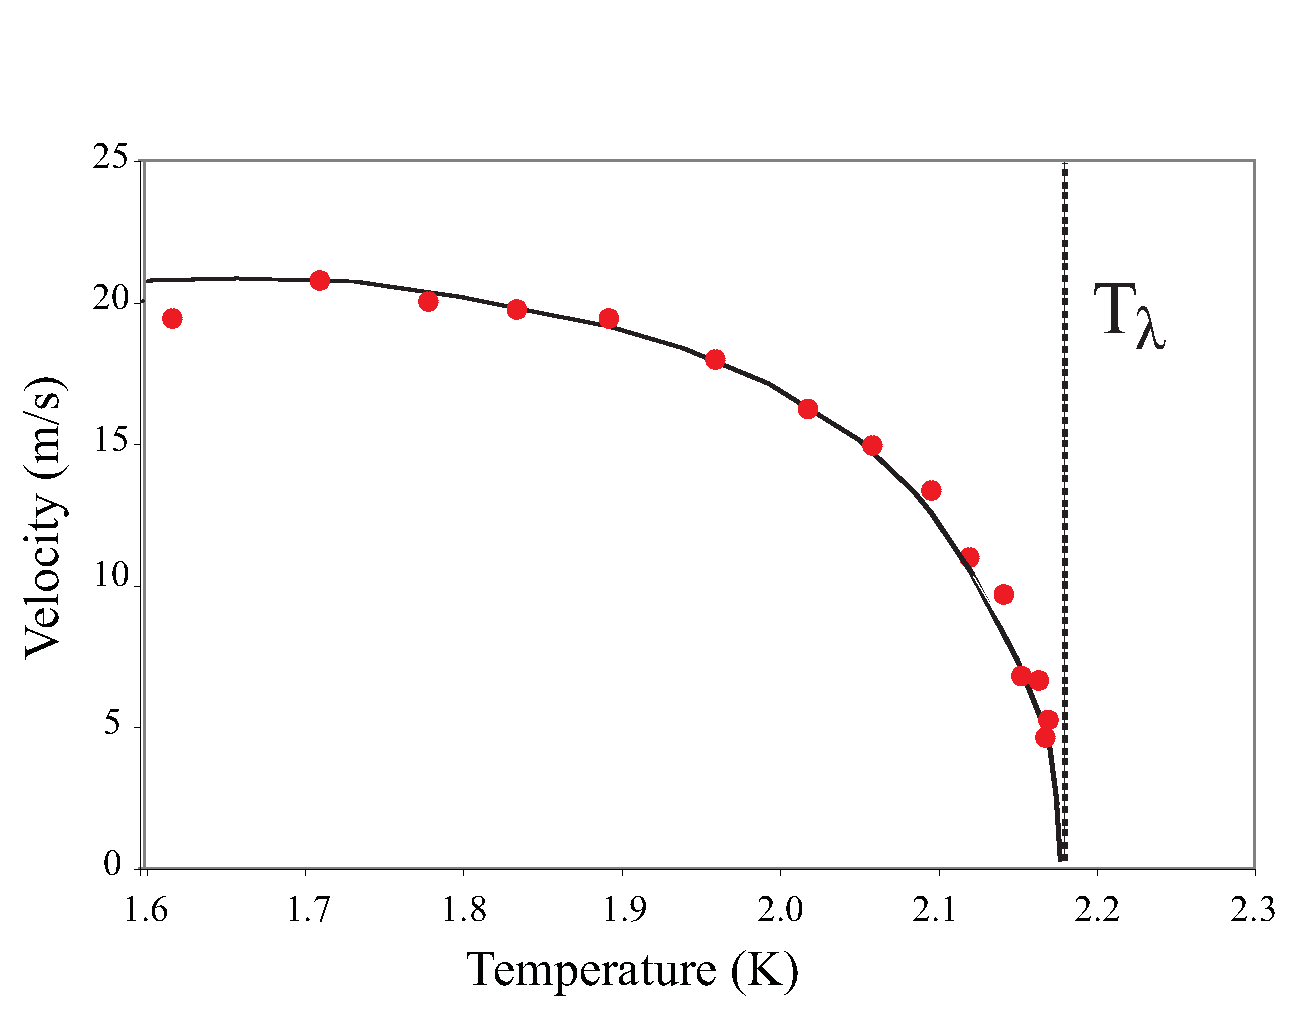
\includegraphics[height=70mm]{./figures/secondsound.eps}
\caption{\small{A plot of the second sound speed verses temperature in He (II).  This data is compared to Peshkov's results.\cite{peshkov} Second sound velocity goes to zero at the transition from He (II) to He (I) enabling a rough estimate of $T_{\lambda}$.}}
\label{fig:secondsound}
\end{center}
\end{figure}

%\footnote{V. Peshkov, "'Second Sound' in Helium II," J. Phys. (Moscow) 8, 381 (1944)}

\subsection{Heat Capacity Analysis}\label{heatcapacityanalysis}
\subsubsection{Temperature Calibration}\label{temperaturecalibration}

%\begin{figure}[htbp]
%\begin{center}
%\includegraphics[height=70mm]{./figures/.eps}
%\caption{\small{}}
%\label{fig:}
%\end{center}
%\end{figure}

\subsubsection{Calculating the Heat Capacity of the Cell}\label{calculatingtheheatcapacityofthecell}

\begin{figure}[htbp]
\begin{center}
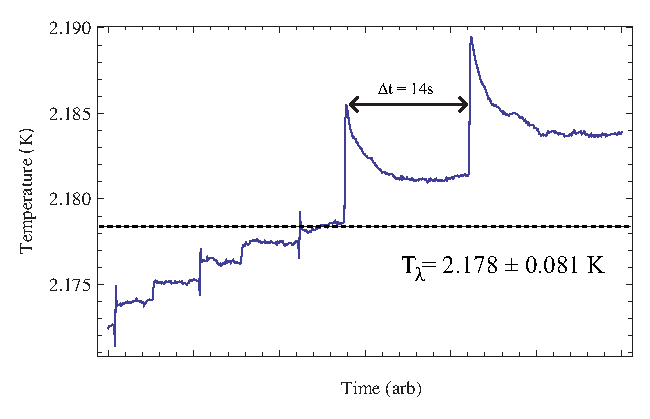
\includegraphics[height=70mm]{./figures/heatingdata.eps}
\caption{\small{A plot of the data from Figure~\ref{fig:rawdata} (b) after being converted from electric potential to temperature using the calibration in Section \ref{temperaturecalibration}.  From this data, $T_{\lambda}$ is determined to be $2.176\pm0.010$ K.}}
\label{fig:heatingdata}
\end{center}
\end{figure}

\begin{figure}[htbp]
\begin{center}
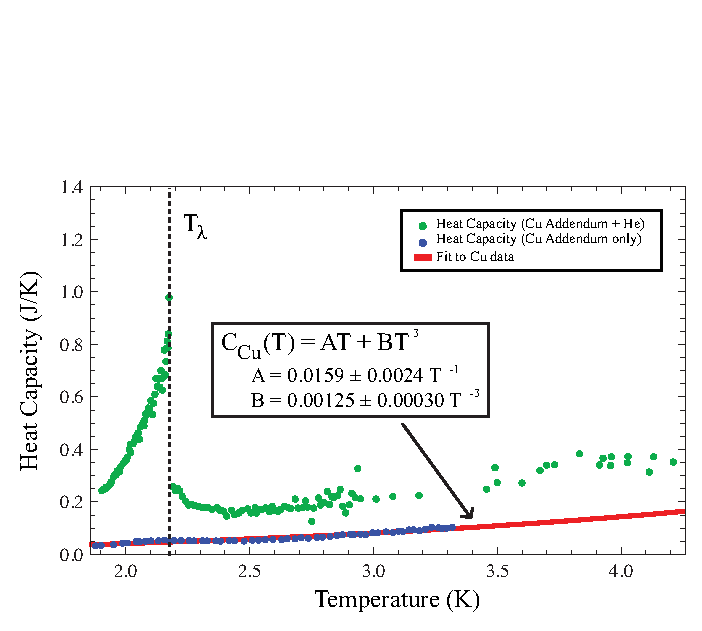
\includegraphics[height=80mm]{./figures/lambdanorm.eps}
\caption{\small{A plot of the heat capacity of the Cu addendum filled with He (II)) and the heat capacity of the evacuated Cu addendum.  A polynomial with cubic and linear terms was fit to the Cu data in order to ultimately remove the addendum's contribution to the heat capacity data.}}
\label{fig:lambdanorm}
\end{center}
\end{figure}

\subsubsection{Calculating the Specific Heat of Superfluid Helium}\label{calculatingthespecificheatofsuperfluidhelium}

\begin{figure}[htbp]
\begin{center}
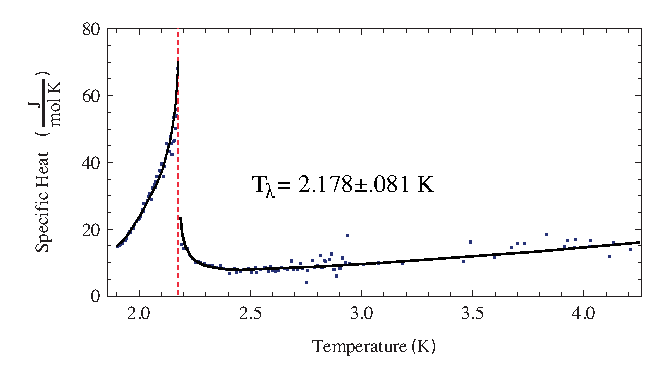
\includegraphics[height=80mm]{./figures/lambdatrans.eps}
\caption{\small{A plot of the specific heat of He(II) verses temperature. The transition from He(I) to He (II) occurs at $T_{\lambda} = 2.176 \pm .010$ K.  The values for specific heat each have a statistical error of $Blah$ J/mol K.}}
\label{fig:lambdatrans}
\end{center}
\end{figure}

